%configurazioni	
	\documentclass[10pt,a4paper]{report}
	\usepackage{graphicx}
	\usepackage[utf8]{inputenc}
	\usepackage{amssymb,amsmath}
	\usepackage{geometry}
	\usepackage[italian]{babel}  
	\usepackage[bookmarks=true]{hyperref}
	\usepackage{bookmark}
	
	
	\geometry{letterpaper}	

\hypersetup{
	pdftitle={Campi elettromagnetici},%
	pdfauthor={Edoardo Contini},%
	pdfsubject={Campi Elettromagnetici},%
	pdfkeywords={},%
	colorlinks=true,%
	linkcolor=blue,%
	linktocpage=true,%
	pageanchor=true
}


\begin{document}

\begin{titlepage}

	\centering
	{\scshape\huge\textbf Politecnico di Milano \par}
	\vspace{0.5cm}

	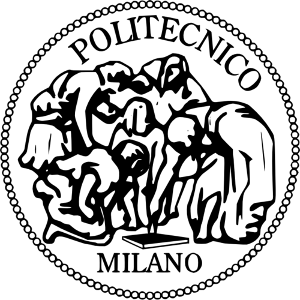
\includegraphics[width=0.15\textwidth]{logo.png}\par\vspace{0.2cm}
	
	{\scshape\small Facoltà di ingegneria\par}
	{\scshape\small Dipartimento di elettronica e informazione\par}
	\vspace{1.5cm}
	{\huge\bfseries Campi Elettromagnetici\par}
	\vspace{1.5cm}
	{\scshape Appunti\par}
	{\scshape\small 2015-2016 \par}
	\vspace{2cm}
	%{\Large\itshape Edoardo Contini\par}
	\vfill
    \raggedleft{Professore: \\ \textit{Michele D'Amico}}	
    \\[1cm]
	
	\raggedright
    {Studente:\\ \textit{Edoardo Contini}
	
	}\vfill
	\raggedleft
	{\large \today\par}
	
	%\raggedright
	%\textit{La risposta è dentro di voi (ma è sbagliata)}.
	%{\\Corrado Guzzanti}
	\end{titlepage}

%\author{Edoardo Contini}


        \newpage
        \null 
        \thispagestyle{empty} 
        \newpage
        
%\maketitle
\tableofcontents
		\newpage
        \null 
        \thispagestyle{empty} 
        \newpage

\pdfbookmark{\contentsname}{Indice}

\chapter{Distribuzioni di carica}

	\section{Conduttori Coassiali}
		\subsection{Tensione tra i conduttori}

		La tensione tra due conduttori coassiali riempiti con dielettrico , sui quali è distribuita una densità di carica superficiale $\rho_l$ opposta si calcola come:
		 \begin{equation}
		 V= \frac {\rho_l}  {2 \pi \epsilon_0} ln ( \frac { r_{out} } { r_{in} } )
		 \end{equation}
	
	\section{Conduttori cilindrici affiancati}

		Il potenziale tra due conduttori cilindrici affiancati su cui è distribuita una densità di carica $\rho_l$ opposta risulta:

		\begin{equation}
		V=\frac{\rho_l}{2 \pi \epsilon_0}{ln(\frac{d^2}{R^+R^-})}
		\label{eq:potenzialebifilari}
		\end{equation}

		La capacità risulta invece:

		\begin{equation}
		C=\frac{2 \pi \epsilon_0}{ln(\frac{d^2}{R^+R^-})}
		\end{equation}

	\section{Distribuzioni di carica lineare}

		\subsection{Potenziale dovuto a distribuzioni di carica lineari}
		E' possibile calcolare il potenziale in punto qualsiasi dello spazio come: 
		\[
		V=\frac{\rho}{2\pi \epsilon}ln(\frac{d_{punto-carica}}{d_{carica-origine}})
		\]

	\section{Cariche puntiformi}

		Il potenziale in un punto P generato da un carica puntiforme, dato dall' integrazione del campo elettrico coulombiano, risulta:

		\[
		V(P)=\frac{Q}{4\pi \epsilon r}
		\]
		Dove:
		\begin{itemize}
		\item "Q" è la carica puntiforme.

		\item "r" è la distanza del punto P\footnote{In cui calcoliamo il potenziale} dalla carica.
		\end{itemize}

\chapter{Metodo delle immagini}	


	\section{Piano conduttore}

	Per annulare il potenziale su un piano conduttore pongo un carica immagine simmetricamente dalla parte opposta rispetto alla carica.

	\section{Linea di trasmissione}

	Esiste una soluzione unica se l'angolo tra i due piani coduttori della linea è$\frac{\pi}{n}$ con n intero.
	Verificata questa condizione dovrò porre $2n-1$ cariche immagine simmetricamente rispetto al sistema.

	\section{Sfera}

	Per annulare il potenziale su una sfera all esterno della quale è posta una carica devo porre una carica immagine a distanza $d'$ dal centro lungo la congiungente tra il centro e la carica esterna tali che:

	\[
	d'=\frac{R^2}{d}
	\]

	Analogamente viene trattato il caso di conduttori cilindrici con distribuzioni di carica lineari.

\chapter{Sorgenti di campo magnetico}

	\section{Spira}
			Il campo magnetico generato da una spira circolare nella direzione assiale\footnote{Asse z} è:

			\begin{equation}
			B=\frac{\mu IR^2}{2(z^2+R^2)^{\frac{3}{2}}}
			\end{equation}

		\subsection{Legge di Faraday-Neumann-Lenz}

		\[
		f.e.m.=Area* \mu \frac{dH}{dt} cos(\theta) 
		\]
		Dove $\theta$ è l'angolo compreso tra la direzione del campo magnetico e il vettore normale alla spira.
	\section{Solenoide}
		\subsection{Campo magnetico in un solenoide}
			Il campo magnetico al centro di un solenoide\footnote{Assumento il solenoide riempito con un materiale con permeabilità magnetica relativa $\mu_r$} è:

			\begin{equation}
			B=\mu_0\mu_rNI
			\end{equation}

			Dove:

			\begin{itemize}
			\item $N$ è il numero di spire del solenoide.
			\item $I$ è la corrente che scorre nel solenoide.
			\end{itemize}

		\subsection{Induttanza solenoide}
				\begin{equation} 
				L=\mu \frac{N^2S}{l}
				\label{eq:induttanza-solenoide}
				\end{equation}

	\section{Conduttore cilindrico}
		Dato un conduttore cilindrico di raggio $R$ e attraversato da un dendità di corrente $J$ possiamo calcolare il campo magnetico in tutto la spazio applicando la legge di ampere e risulta:

		\begin{itemize}
		\item Soluzione interna: $H_\phi(R)=\frac{jR}{2}$ 
		\item Soluzione esterna: $H_\phi(R)=\frac{I}{2\pi R}$

		\end{itemize}

\chapter{Linee di Trasmissione}

	\section{Capacità}

	
		\subsection{Linee Coassiali}
				\begin{equation}
				C=\frac{2\pi \epsilon_0 \epsilon_r} {ln (\frac { r_{out}} {r_{in} } )}
				\end{equation}

				Se la linea è rimepita con diverse sezioni di circonferenza di dielettrici, questa puo essere modellizata come il parallelo di due capacità sommate pesandole sulla percentuale di volume occupata dai rispettivi dielettrici.
			
				Se la linea è riempita con dielettrici diversi coassiali, si puo considerare come due coassiali in serie e la capacità risulta come capacità in serie.\footnote{Si ricordi invece che il calcolo dell'induttanza rimane invariato}


		\subsection{Linee Bifilari}

			Utilizzando l'approssimazione dei conduttori sottili si può scrivere che la capacità per unità di lunghezza è data dal rapporto fra la carica per unità di lunghezza e la 
			differenza di potenziale tra i due fili\footnote{vedi la ~\ref{eq:potenzialebifilari}}.
			

			\begin{equation}
			C=\frac{\rho_l 2 \pi \epsilon_0}{\rho_l ln(\frac{d^2}{R^-R^+})}
			\label{eq:capacitabifilare}
			\end{equation}



		\subsection{Microstrisce}

	

	 		Se la linea è costituita da tratti riempiti con dielettrico di diversa natura, la linea può essere modellizzata come più capacità in parallelo calcolate come:

	 		\begin{equation}
			C=\epsilon_0 \epsilon_r\frac{w}{h}	 			
	 		\end{equation} 
	 		dove:
	 		\begin{itemize}
	 		\item $w$ è la lunghezza del settore di linea considerato.
	 		\item $h$ è la distanza tra le strisce
	 		\end{itemize}


	\section{Induttanza}

		\subsection{Linee coassiali}

			Per il calcolo dell’induttanza non è necessario tenere conto della presenza del dielettrico
			poiché questa è indipendente da esso e quindi è pari a quella in aria.
		
			\begin{equation}
				L=\frac{\mu_0 \epsilon_0}{C_0}=\frac{\mu_0 \epsilon_0 ln (\frac { r_{out}} {r_{in} } )}{2\pi \epsilon_0}
			\end{equation}



		\subsection{Linee bifilari}

		Ricordando la ~\ref{eq:capacitabifilare} e la relazione $L=\frac{\mu_0 \epsilon_0}{C_0}$ è immediato calcolare l'induttanza della linea.

		\subsection{Microstrisce}
			
			Per il calcolo dell’induttanza, analogamente a quanto detto per la linea coassiale, non è necessario tenere conto della presenza del dielettrico
			poiché questa è indipendente da esso e quindi è pari a quella in aria.
		
			\begin{equation}
				L=\frac{\mu_0 \epsilon_0}{C_0}=\mu_0 \frac{h}{w}
			\end{equation}
	


	\section{Impedenza caratteristica}

			L'impedenza caratteristica di una linea di trasmissione è il rapporto dei moduli della tensione e della corrente che si propagano in una linea distribuita in una singola direzione, in assenza di riflessioni.

			\begin{equation}
				Z_c=\sqrt{\frac{L}{C}}
			\end{equation}

	\section{Spessore pelle}
			Lo spessore pelle indica la profondità di penetrazione del campo in un conduttore.
			\begin{equation}
			\delta=\frac{1}{	\sqrt{\pi \sigma f \mu_o}}
			\end{equation}

	\section{Velocità di fase}
			 La velocità di fase può essere visualizzata come la velocità di propagazione di una cresta dell'onda ma non coincide necessariamente con la velocità di propagazione di un segnale (che è più propriamente descritta dalla velocità di gruppo) e quindi può essere più alta della velocità della luce senza violare la relatività ristretta.
			\begin{equation}
				v_f=\frac{1}{\sqrt{LC}}
			\end{equation}

	\section{Resistenza}

		\subsection{Linee Coassiali}

			La resistenza per unità di lunghezza si calcola come:

			\begin{equation}R=\frac{1}{\sigma \delta p}=\frac{1}{\sigma \delta 2 \pi}(\frac{1}{r_{out}}+\frac{1}{r_{in}})\end{equation}
			dove:
			
			\begin{itemize}
			\item $\sigma$ è la conducibilità del conduttore.
			\item $\delta$ è lo spessore pelle.
			\item $p$ è il perimetro della sezione nel conduttore interessata dal passaggio di corrente.
			\end{itemize}

		\subsection{Linee bifilari}

				La resistenza per unità di lunghezza per una linea bifilare si calcola come:

				\begin{equation}R=\frac{2w}{\sigma \delta}\end{equation}
				dove:
				
				\begin{itemize}
				\item $\sigma$ è la conducibilità del conduttore
				\item $\delta$ è lo spessore pelle
				\item $w$ è la lunghezza della linea
				\end{itemize}

		\subsection{Microstrisce}

			Analogamente ai casi precedenti si calcola le resistenza considerando il solo spessore di conduttore ricavato con lo spessore pelle e la larghezza della microstriscia.\footnote{Il calcolo è quindi analogo alla linea coassiale sostiuendo il perimetro con la larghezza della microstriscia.}

	\section{Conduttanza per unità di lunghezza}

			\begin{equation}
			g=\frac{\sigma C}{\epsilon}
			\end{equation}

	%g=\frac{\sigma_d * Area}{h}	= \sigma_d \frac{w}{h}




	\section{Costante di attenuazione dovuta ai conduttori}
	
			La costante di attenuazione dovuta alla conducibilità finita dei conduttori si trova da:
			\begin{equation}
			\alpha_c=\frac{R}{2Z_c}
			\end{equation}
		
	\section{Costante di attenuazione dovuta al dielettrico}
	
			L'attenuazione dovuta alle perdite\footnote{per unità di lunghezza.} nel dielettrico è conseguenza di una conducibiltà non nulla di materiali non ideali.

			\begin{equation}
			\alpha_d=\frac{g}{2Y_c}
			\end{equation}

	\section{Attenuazione totale}

			\begin{equation}
			A=\alpha L
			\end{equation}
			Dove:
			\begin{itemize}
			\item L è la lunghezza totale della linea.
			\item $\alpha=\alpha_d+\alpha_c$ è la costante di attenuazione totale che tiene conto sia delle perdite nel dielettrico che nei conduttori.
			\end{itemize}

	\section{Conversione Np-dB}

	\[
	1\frac{Np}{m}=8,868\frac{dB}{km}
	\]
	
	\section{Potenza associata all'onda progressiva}

			\begin{equation}
			P=\frac{1}{2}\frac{|V^+|^2}{Z_0}=\frac{1}{2}|I^+|^2 Z_0
			\end{equation}

	\section{Potenza dissipata}

			\begin{equation}
			P_{diss,COND}=\frac{1}{2}|I_{max}|^2 r
			\end{equation}

			\begin{equation}
			P_{diss,DIEL}=\frac{1}{2} g V^2
			\end{equation}

	\section{Campo magnetico massimo}
	
 			Ricordando la legge di Ampere conoscendo la corrente massima si può calcolare i campo magnetico massimo come:

			\begin{equation}
			2 \pi a |H_{max}| = |I_{max}|
			\end{equation}

	\section{Costante di fase}
			%		    \subsection{Microstrisce}
			\begin{equation}
				\beta=\omega \sqrt{LC}=2 \pi f \sqrt{LC}
			\end{equation}
		
\chapter{Propagazione in multistrato}

	\section{Impedenza intrinseca}

		L'impedenza intrinseca per la propagazione in un mezzo dielettrico\footnote{In assenza di perdite} si calcola come:

		\begin{equation}
		\eta=\frac{\eta_0}{\sqrt{\epsilon_r}}
		\end{equation}

		Dove $\eta_0=377\Omega$ è l'impedenza caratteristica del vuoto.

		Se il dielettrico presenta una conducibilità equivalente non nulla l'impedenza instrinseca risulta:

		\begin{equation}
		\eta=\frac{j\omega\mu}{\sqrt{-\omega^2\mu\epsilon+j\omega\mu\sigma_{eq}}} [  \Omega  ]
		\end{equation}
		Dove la conducibilità equivalente si calcola come:

		\begin{equation}
		\sigma_{eq}=\omega \epsilon''
		\end{equation}
		Risulta $\epsilon=\epsilon'+j\epsilon''$.
		
		I coefficienti $\epsilon'$ e $\epsilon''$ vengono dati tramite il parametro\footnote{In cui si ricorda che la $\delta$ non ha nulla a che fare con lo spessore pelle.} $tan\delta=\frac{\epsilon''}{\epsilon'}$.

	\section{Lunghezza d'onda in mezzi dielettrici}
		Una radiazione che si propoaga in un mezzo con constante dielettrica diversa da quella del vuoto subisce una variazione della lunghezza d'onda:

		\begin{equation} 
		\lambda = \frac {\lambda_0} {\sqrt {\epsilon_r} }
		\end{equation} 

	\section{Equivalente in linea di trasmissione}

		
		La propagazione in un mezzo multistrato può essere modellizata come una linea di trasmissione in cui i vari spezzoni di linea hanno impedenza caratteristica uguale all'impedenza intrinseca del mezzo in cui si propagano.	
		Si puo quindi studiare il problema con l'utilizzo della carta di Smith.

	\section{Condizioni al contorno per il campo elettrico}

		Nell interfaccia tra mezzi con costante dielettrica diversa abbiamo che:
		\begin{equation}
		E_{t1}=E_{t2} 
		\end{equation}
		cioé $\epsilon_1 D_{t1} = \epsilon_2 D_{t2}$.
		Mentre per la componente normale si ha:
		\begin{equation}
		D_{n1} = D_{n2}
		\end{equation}
		cioè:
		\[
		\frac{E_{n1}}{\epsilon_1}=\frac{E_{n2}}{\epsilon_2}
		\]

	\section{Condizioni al contorno per il campo magnetico}
		Nell'interfaccia tra mezzi con permeabilità magnetica diversa si ha:
		\begin{equation}
		B_{n1}=B_{n2} 
		\end{equation}
		cioé $\mu_1 H_{n1} = \mu_2 H_{n2}$.
		Mentre si conserva la componente tangenziale\footnote{Assumendo nulla la densità superficiale di corrente all'intefaccia. Tenendone conto risulterebbe: $J_s=H_{t1}-H_{t2}$}.
		\begin{equation}
		H_{t1}=H_{t2}
		\end{equation}

	\section{Campo elettrico e campo magnetico}

	Conoscendo la densità di potenza propagante possiamo calcolare il modulo di campo elettrico e magnetico come:

	\[
	S=\frac{E^2}{2\eta_{mezzo}}=\frac{H^2}{2}\eta_{mezzo}
	\]

	\section{Vettore di Poynting}
		Per una radiazione propagante in un mezzo possiamo calcolare il valore medio del vettore di Poynting come:
		\begin{equation}
		\overline{S_{avg}}=\frac{A^2}{2\eta}
		\end{equation}
		Dove A è l'ampiezza del campo elettrico.
		E' possibile calcolare anche il valore istantaneo che risulta:

		\begin{equation}
		S_{ist}=\frac{A^2}{\eta}\cos^2(\omega t)
		\end{equation}
	
	\section{Legge di snell}

	La legge di snell viene utilizzata per studiare il caso semplificato di impedenza normale.


\chapter{Incidenza obliqua}

	Avendo una radiazione incidente con angolo obliquo su un intefaccia tra dielettrici diversi per studiare la trasmissione nel mezzo 2 è necessario scomporre la radiazione in propagazione trasverso elettrica e trasverso magnetica.

	\section{Angolo di trasmissione}
	Si ricava , utilizzando la legge di Snell:
	\begin{equation}
	\theta_T=\arcsin(\frac{\sqrt{\epsilon_{r1}}}{\sqrt{\epsilon_{r2}}}\sin(\theta_i)
	\end{equation} 
	
	\section{Condizioni limite}

		\subsection{T.I.R.}
			La condizione di trasmissione totale interna implica un coefficiente di riflessione $\Gamma$ unitario.

			\textbf{NOTA:}

			Si ricordi che in caso si TIR il fatto che non ci sia potenza trasmessa nel mezzo 2 non implica il fatto che i campi siamo nulli.
			L'intensità dei campi nel mezzo 2 possono essere calcolati attraverso la valutazione dell'onda evanescente:


		
		\subsection{Angolo di Brewster}

			Nel caso di angolo di incidenza uguale all'angolo di Brewster\footnote{Vedi la ~\ref{eq:brewster}} abbiamo trasmissione totale nel mezzo 2, cioe $\Gamma=0$.

	\section{Modo trasverso elettrico}

		\subsection{Impedenza caratteristica TE}
			\begin{equation}
			\eta_{TE}=\frac{\eta_0}{\sqrt{\epsilon_r}\cos(\theta)}
			\end{equation}

		\subsection{Coefficiente di riflessione}
			Conoscendo le impedenze intrinseche posso calcolare il coefficiente di riflessione per il modo TE come:

			\[
			\Gamma_{TE}=\frac{\eta_{TE1}-\eta_{TE2}}{\eta_{TE1}+\eta_{TE2}}
			\]
		%	 Si noti che questo coefficiente di riflessione è valido solo per la componente tangente del campo elettrico.

			 \textbf{NOTA:}
			 \\ 
			 Nello studio della propagazione di modi trasverso elettrici il coefficiente di trasmissione $\Gamma_{TE}$ si può utilizzare solo per il calcolo del campo elettrico e non del campo magnetico , il quale si potrà poi essere calcolato utilizzando la ~\ref{eq:campo-magnetico}.

		\subsection{Potenza trasmessa}

			Per calcolare la potenza trasmessa nel mezzo 2:
			\begin{itemize}
			\item Proietto la potenza incidente sull'asse normale all'intefaccia.

			\begin{equation}
			S_{inc_\perp}=S_{inc}\cos(\theta_i)
			\end{equation}

			\item Tramite il coefficiente di trasmissione calcolo la componente normale della potenza trasmessa:
			\begin{equation}
			S_{t_\perp}=S_{inc_\perp}(1-|\Gamma_{TE_\perp}|^2)
			\end{equation}

			\item Conoscendo l'angolo di trasmissione e la componente normale è possibile calcolare la potenza totale trasmessa nel mezzo 2.

			\begin{equation}
			S_{t}=\frac{S_{t_\perp}}{\cos(\theta_t)}
			\end{equation}
			\end{itemize}
		\subsection{Campo elettrico}

			Per valutare il campo elettrico in un punto dello spazio devo valutare diversi coefficienti di propagazione:
			\[
			\gamma=j\omega\sqrt{\mu\epsilon}\]

			Da cui ricavo le due componenti:

			\[
			\gamma_x=\gamma\sin(\theta)
			\]

			\[
			\gamma_y=\gamma\cos(\theta)
			\]

			E' quindi possibile esprimere il campo elettrico propagante\footnote{Valido sia per modi TE che TM} nel mezzo come:
			
			\[
			E(x,y)=E(0,0)e^-{j\gamma_x x}e^-{j\gamma_y y}
			\]
		
			\textbf{NOTA:}

			Si ricordi che studiando il modo trasverso elettrico il coefficiente di riflessione va applicato alla sola componente tangente del campo elettrico\footnote{Unica presente in modo TE.}.
			
	\section{Modo trasverso magnetico}

			\subsection{Impedenza instrinseca TM}

				\begin{equation}
					\eta_{TM}=\frac{\eta_0}{\sqrt{\epsilon_r}}\cos(\theta)
				\end{equation}

			\textbf{NOTA:}

			Si ricordi che studiando il modo trasverso magnetico il coefficiente di riflessione $\Gamma$ va utilizzato per calcolare la componente di campo elettrico trasmesso normale all'interfaccia.
			Ricavando poi con la legge di Snell l'angolo di trasmissione e conoscendo la componente normale posso trovare il campo trasmesso totale.

		\subsection{Coefficiente di riflessione}
			Conoscendo le impedenze intrinseche posso calcolare il coefficiente di riflessione per il modo TM come:

			\[
			\Gamma_{TM}=\frac{\eta_{TM1}-\eta_{TM2}}{\eta_{TM1}+\eta_{TM2}}
			\]
		
			 
			 \textbf{ NOTA: }
			 
			 Nello studio della propagazione di modi trasverso elettrici il coefficiente di trasmissione $\Gamma_{TM}$ si può utilizzare solo per il calcolo del campo magnetico e non del campo elettrico , il quale si potrà poi essere calcolato utilizzando la ~\ref{eq:campo-elettrico}.

		\subsection{Potenza trasmessa}

			Per calcolare la potenza trasmessa nel mezzo 2:
			
			\begin{itemize}
			
			\item Proietto la potenza incidente sull'asse normale all'intefaccia.
			\begin{equation}
			S_{inc_\perp}=S_{inc}\cos(\theta_i)
			\end{equation}

			\item Tramite il coefficiente di trasmissione calcolo la componente normale della potenza trasmessa:
			\begin{equation}
			S_{t_\perp}=S_{inc_\perp}(1-|\Gamma_{TM_\perp}|^2)
			\end{equation}

			\item Conoscendo l'angolo di trasmissione e la componente normale è possibile calcolare la potenza totale trasmessa nel mezzo 2.
			\begin{equation}
			S_{t}=\frac{S_{t_\perp}}{\cos(\theta_t)}
			\end{equation}
			

			\end{itemize}
		

		\subsection{Campo magnetico}

			Per valutare il campo magnetico in un punto dello spazio devo valutare diversi coefficienti di propagazione:
			\[
			\gamma=j\omega\sqrt{\mu\epsilon}\]

			Da cui ricavo le due componenti:

			\[
			\gamma_x=\gamma\sin(\theta)
			\]

			\[
			\gamma_y=\gamma\cos(\theta)
			\]

			E' quindi possibile esprimere il campo magnetico propagante\footnote{Valido sia per modi TE che TM.} nel mezzo come:
			
			\[
			H(x,y)=H(0,0)e^-{j\gamma_x x}e^-{j\gamma_y y}
			\]
		

		\section{Onde incidenti generiche}

		In presenza di un onda non solamente TM o TE si studiano i due tipi di modi separatamente e si compongono alla fine con la somma quadratica\footnote{Ciò vale sia per le potenze che per i campi.}:

		\[
		S_{t}=\sqrt{S_{t_{TE}}^2 +S_{t_{TM}}^2 }
		\]

\chapter{Adattamento}

	\section{Adattatore con nutralizzatore}

		L'adattatore con neutralizzatore è un tratto di linea da inserire tra il carico e la fine dell'adattatore lambda quarti ed è utilizzato e dimensionato in modo che porti all'interfaccia del $\frac{\lambda}{4}$ un impendenza reale pura.

	\section{Adattatore lambda quarti}
		
		L'adattatore lambda quarti è un tratto di linea con impedenza caratteristica e lunghezza da dimensionare opportunamente che viene inserito per adattare il carico alla linea.

		\subsection{Impedenza caratteristica}
				Muovendosi sulla carta di smith è necessario trovare le impedenze viste ad entrambe le interfacce dell'adattore.

				\begin{equation}
				\eta_{\frac{\lambda}{4}}=\sqrt{\eta_{dx}\eta_{sx}}
				\end{equation}

		\subsection{Lunghezza della linea}
				Imponendo le condizioni di interferenza distruttiva tra le onde riflesse alle 2 interfaccie si trova che la lunghezza del tratto di linea da inserire deve essere un quarto della lunghezza d'onda:\footnote{Eventualmente da modificare a seconda della costante dielettrica del mezzo in caso di linea equivalente ad un multistrato.}
				\begin{equation}
				L_s= \frac {\lambda} {4}
				\end{equation}

	\section{Stub parallelo}

		Dimensionando l'adattamento con stub parallelo è necessario lavorare con la carta delle ammettenze\footnote{Si ricordi che nella carta delle ammettenze il corto circuito si trova a destra.}, ogni impedenza $Z$ va quindi trasformata in ammettenza come: $Y=\frac{1}{Z}$

		\subsection{Corto circuito}
				
			Per l'adattamento con stub parallelo si trova l'ammettenza del carico $Y_L=\frac{1}{Z_L}$ e la si normalizza per l'ammettenza caratteristica del tratto di linea attraverso cui ci si sta muovendo: $\overline{Y_{LL}}=\frac{Y_L}{Y_O}$.


			A questo punto riportando $\overline{Y_{LL}}$ sulla carta delle ammetenze , ruoto fino ad individuale i punti di intersezione con la circonferenza unitaria

			Indivuduata la parte immaginaria dell'impedenza , partendo dal corto circuito ruoto sulla circonferenza esterna della carta di smith\footnote{Circonferenza a parte reale.} ruoto fino al punto a parte immaginaria opposta rispetto a quella dell'impedenza dovuta al carico e determino cosi la lunghezza dello stub.

		\subsection{Circuito aperto}

		Il procedimento per il dimensionamento di stub parallelo a circuito aperto è analogo a quello utilizzato per lo stub parallelo a corto circuito con l'unica differenza che nel determinare la lunghezza dello stesso la rotazione sulla carta di Smith deve partire dal punto ad impedenza infinita, cioè ammettenza nulla\footnote{Al contrario del procedimento adottato per gli stub corto circuito.}.

	\textbf{NOTA:}

	Si ricordi che sarebbe possibile utilizzare anche la carta di Smith delle impedenze per trattare stub parallelo, bisognerebbe però avere l'accortezza di comporre le impedenze in parallelo, non in sommandole in serie come è possbile fare con le ammettenze.

	
	\section{Stub serie}

	 	Il metodo di dimensionamento degli stub serie è duale a quello per gli stub parallelo. E' però necessario usare la carta di Smith delle impedenze, sommando queste tra loro.

		
	\section{Adattamento con carico reattivo}

		Analogamente a quanto visto per gli adattatori lambda-quarti e stub parallelo e serie, un altro metodo di adattamento del carico consiste nell'inserimento in linea di un carico reattivo\footnote{Capacità o induttanza.}.

		Analogamente al discorso fatto per gli stub il carico reattivo puuò essere aggiunto in serie o in parallelo.

		\subsection{Serie}
			Con un approccio analogo a quello utilizzato per gli stub serie si lavora con la carta di Smith delle impedenze.
		\subsection{Parallelo}
					Con un approccio analogo a quello utilizzato per gli stub parallelo si lavora con la carta di Smith delle ammettenze.

	\section{Tensione su carico adattato}

	Per trovare la tensione sul carico adattato si utilizza l'espressione:

	\[
	P_d= \frac {V_{load}^2}{2} Re\{ Y_{load}] \}
	\]
	Poichè tutta la potenza disponibile viene trasferita al carico.

	Per trovare invece la corrente che fluisce nel carico si utilizza la legge di ohm:

	\[
	I=\frac{V}{|Z_{load}|}
	\]

\chapter{Propagazione in linea}



	\section{Potenza}
		In caso di adattamento abbiamo che tutta la potenza disponibile è trasferita al carico e in particolare vale:
			
			\begin{equation}
			P_L=P_d=(\frac{V_g}{2})^2\frac{1}{2Z_g}=\frac{V_g^2}{8Z_g}
			\end{equation}

			La potenza trasmessa al carico può anche essere calcolata tramite il vettore di pointing e il coefficiente di riflessione:

			\begin{equation}
			S_{tr}=S_{inc}(1-|\Gamma|^2)
			\end{equation}

			Analogo discorso si può fare con la potenza.
			La potenza trasferita al carico risulta essere:

			\begin{equation}
			P_{load}=P_{inc}(1-|\Gamma|^2)
			\end{equation}
	\section{Tensione al carico}

			\begin{equation}
			P_L=\frac{V_{L}}{2}Re\{Y_L\}
			\label{eq:tensionealcarico}
			\end{equation}

			Tale relazione può essere utilizzata per ricavare la tensione in ogni punto della linea considerando la potenza e l'impedenza viste ad una determinata interfaccia.
	\section{Corrente al carico}


			\begin{equation}
			P_L=\frac{I_{L}}{2}Re\{Z_L\}
			\label{eq:correntealcarico}
			\end{equation}
			Come per la \ref{eq:tensionealcarico} tale relazione può essere utilizzata in ogni punto della linea.
	\section{Legge di Ohm}

	Possiamo utilizzare la legge di Ohm per ricavare la corrente conoscendo la tensione o viceversa , utilizzando il modulo dell impedenza come segue:

	\[
	I_L=\frac{V_L}{|Z_L|}
	\]

			Come per la \ref{eq:tensionealcarico} e la \ref{eq:correntealcarico} tale relazione può essere utilizzata in ogni punto della linea.


	\section{Attenuazione}

		Se in linea abbiamo delle perdite e conosciamo il coefficiente di attenuazione $\alpha$, sappiamo che la potenza si propaga come:
		\begin{equation}
		P(x)=P_0e^{-2 \alpha x}
		\end{equation}

		Si ricordi come in presenza di perdite in linea la potenza erogata risulta uguale alla somma della potenza dissipata lungo la linea e alla potenza trasferita al carico:

		\begin{equation}
		P_{erogata}=P_{diss}+P_{load}
		\end{equation}

	\section{Rapporto d'onda stazionaria}

	\begin{equation}
	ROS=\frac{|V_{max}|}{|V_{min}|}=\frac{|V_o^+|(1+|\Gamma|)}{|V_o^+|(1-|\Gamma|)}
	\end{equation}

	\section{Linee attenuative}

		\subsection{Coefficiente di riflessione al carico}

		\[
		\Gamma_L=\frac{Z_C-Z_L}{Z_C+Z_L}
		\]
		\subsection{Coefficiente di riflessione attenuato}
		Lungo la linea con perdite il coefficiente di riflessione viene attenuato come:
		\[
		\Gamma_{attenuato}=\Gamma_L e^{-2\alpha L}
		\]
		Riportando sulla carta di Smith il coefficiente di riflessione attenuato possiamo ottenere l'impedenza vista all'interfaccia di ingresso, da cui è possibile ricavare il coefficiente di riflessione in ingresso:

		\[
		\Gamma_{in}=\frac{Z_G-Z_{in}}{Z_G+Z_{in}}
		\]

		Da cui conoscendo la potenza incidente possiamo ricavare la potenza immessa in linea come:

		\[
		P_{in}=P_d(1-|\Gamma_{in}|^2)
		\]

		\subsection{Tensione all'interfaccia di ingresso}

		Conoscendo l'impedenza di ingresso possiamo applicare un partitore di tensione come:

		\[
		V_{in}=V_g|\frac{Z_{in}}{Z_{in}+Z_g}|
		\]
		\textbf{NOTA:}

		Si faccia attenzione al fatto che trattando potenze propaganti in linea è necessario considerare solo le parti reali delle impedenze o delle ammettenze.

\chapter{Guide d'onda}
		
	\section{Modo trasverso elettrico}

		\subsection{Campo elettrico}
				\begin{equation}
				E_y= E_0e^{-j\beta z}+E_0 \Gamma e^{j \beta z}=E_0(e^{-j \beta z}+\Gamma e^{j \beta z}) =E_0(1 - \Gamma)e^{-j \beta z} + E_0 \Gamma \cos(\beta z)
				\end{equation}

		\subsection{Campo magnetico}

				\begin{equation}
				H_{max}=H^+(1+|\Gamma|)=\frac{E^+}{\eta_{TE_{10}}}{(1+|\Gamma|)}
				\end{equation}

		\subsection{Frequenza di work}

				\begin{equation}
				f_w=\frac{\frac{c}{2a}+\frac{c}{2b}}{2}
				\end{equation}

				Si ricordi che questa relazione è valida solo nel caso in cui $b<a<2b$.

		\subsection{Frequenza di cut}
	
				La frequenza di cut è la frequenza limite di funzionamento monomodale
				\begin{equation}
				f_c=\frac{c}{2a}
				\end{equation}
				Dove $a$ è il lato piu lungo della guida.

		\subsection{Lunghezza d'onda in setto di dielettrico}

			\begin{equation}
			\lambda_{TE}=\frac{1}{\sqrt{\epsilon_r}}\frac{\lambda}{\sqrt{1- (\frac{f_c}{\sqrt{\epsilon_r}f_w})^2}}
			\end{equation}

		\subsection{Impedenza modale nel vuoto}

				\begin{equation}
				\eta_{TE_{vuoto}}=\frac{\eta_0}{ \sqrt{ 1- ( \frac {f_{cut}} {f_{work}} )^2 } }
				\end{equation}
		\subsection{Impedenza modale nel setto di dielettrico}

				\begin{equation}
				\eta_{TE_{setto}}=\frac{\eta_0}{\sqrt{\epsilon_r} \sqrt{ 1- ( \frac {f_{cut}} {\sqrt{\epsilon_r} f_{work}} )^2 } }
				\end{equation}

		\subsection{Coefficiente di riflessione}

			\[
			\Gamma_{TE}=\frac{\eta_{TE_{vuoto}}-\eta_{TE_{setto}}}{\eta_{TE_{vuoto}}+\eta_{TE_{setto}}}
			\]
		\subsection{Campo elettrico nel setto di dielettrico}
		\[
		E_{max}=E_g(1+|\Gamma|)
		\]

		\[
		E_{min}=E_g(1-|\Gamma|)
		\]


		\subsection{Potenza in guida}
				\begin{equation}
				P_0=\frac{E_0^2}{4\eta_{TE}}ab
				\end{equation}
				Si noti che nel caso di inserimento di un setto $\lambda/2$ in guida abbiamo un onda viaggiante , l'inviluppo del campo elettrico è quindi costante tranne nel setto di dielettrico, in cui è simmetrico rispetto al punto medio.
				Nel caso di $\frac{\lambda}{2}$ si ha che $E_0$ coincide con $E_{max}$.
		

\chapter{Propagazione di onde piane}

	\subsection{Campo elettrico}

		\begin{equation}
		E=H\eta
		\label{eq:campo-elettrico}
		\end{equation}
		

	\subsection{Campo magnetico}
		\begin{equation}
		H=\frac{E}{\eta}
		\label{eq:campo-magnetico}
		\end{equation}
	

	\subsection{Potenza propagante}


		\begin{equation}
		P=S*Area=\frac{EH}{2}*Area=\frac{E^2}{2\eta}*Area=\frac{H^2\eta}{2}*Area
		\label{eq:potenza-propagante}
		\end{equation}
	
	\subsection{Potenza dissipata}

		La potenza dissipata in un mezzo si calcola come la differenza tra la potenza finale e quella iniziale.
		\begin{equation}
			P_{diss}=P_{finale}-P_{iniziale}
			\label{eq:potenza-dissipata}
		\end{equation}
	
	\subsection{Costante di propagazione d'onda}
		\[
		\gamma=\sqrt{j\omega\mu(\sigma+j\omega\epsilon_0\epsilon_r)}
		\]
	\subsection{Impedenza intrinseca}
		\[
		\eta=\sqrt{\frac{j\omega\mu}{\sigma+j\omega\epsilon_0\epsilon_r}}
		\]
		

	\subsection{Angolo di Brewster}

	L'angolo di Brewster è l'angolo di incidenza a cui abbiamo trasmissione totale:
	\[
	\sin(\theta_B)=\sqrt{\frac{\epsilon_2}{\epsilon_2+\epsilon_1}}
	\label{eq:brewster}
	\]




	\subsection{Propagazione}
	Ricordiamo la propagazione di un onda piana in un mezzo:
	

	\[
	E(x)=E_0e^{-\gamma x}
	\]
	
	Da cui usando la ~\ref{eq:campo-magnetico} possiamo calcolare il campo magnetico, e usando la ~\ref{eq:potenza-propagante} e la ~\ref{eq:potenza-dissipata} possiamo calcolare la potenza dissipata nel volume considerato.


	\subsection{Polarizzazione}

	Conoscendo le componenti x e y del campo elettrico è possibile individuale la polarizzazione dell'onda.

	\raggedright	{1) Se i moduli della componente x e y sono diversi\footnote{A meno che le due componenti non abbiamo sfasamento o nullo o uguale a $\pi$.}:}

	\begin{itemize} 
	\item \textbf{Polarizazzione ellittica}
	\end{itemize}
	\raggedright{	2) Se le due componenti sono uguali in modulo, si disegnano sul piano di Gauss i fasori corrispondenti ai campi $E_x$ ed $E_y$.}
	\begin{itemize}
	\item \textbf{Polarizzazione lineare}: se i due vettori hanno la stessa fase\footnote{Sono sovrapposti sul piano di Gauss} o sono sfasati di $\pi$.
	\item \textbf{Polarizzazione Circolare} se i due vettori hanno uno sfasamento.
	\end{itemize}
		
	Rimane ora da determinare la tipologia di polarizzazione circolare.
	
	\raggedright{3) Individuiamo il senso di rotazione:}

	\begin{itemize}

	\item Antiorario: se abbiamo un onda propagante ($e^{-\beta z}$)
	\item Orario: se abbiamo un onda antipropagante ($e^{+\beta z}$)

	\end{itemize}
	\raggedright{4) Dobbiamo far ruotare uno dei due vettori, tenendo fermo l'altro, in modo da chiudere l'angolo convesso\footnote{$<180$} formato dai due.}

	\raggedright{	5) Determiniamo ora la polarizzazione secondo il seguente schema:}

	\begin{itemize}
	\item Polarizzazione Circolare sinistra: se è il vettore $x$ a muoversi verso $y$ 
	\item Polarizzazione Circolare destra: se è il vettore $y$ a muoversi verso $x$ 
	\end{itemize}	


	\section{Riconoscimento onde TEM}
	Affinchè un'onda possa essere chiamate onda TEM devono verificarsi le seguenti:

	\begin{itemize}

	\item Campo elettrico e magnetico siano in fase 

	\item Campo elettrico e campo magnetico siano proporzionali come $E=\eta H$

	\item Campo elettrico e campo magnetico devono essere perpendicolari tra loro e l'onda deve propagarsi su una terza direzione a loro perpendicolare

	\end{itemize}



\chapter{Antenne}
		\textbf{Formula generale\footnote{Valida per tutti i tipi di antenne.}}
		\begin{equation}
		\frac{G}{A_e}=\frac{4\pi}{\lambda^2}
		\end{equation}
	    Dove G è il guadagno che si calcola come $G=\mu D$\footnote{Dove $D=\frac{S_{reale}}{S_{isotropa}}$ è la direttività.}.

	    Il
	 \section{Dipoli elettrici in trasmissione}

		\subsection{Campo elettrico trasmesso}

		Il campo elettrico radiale è un campo vicino che decade a distanze maggiori di $2\lambda$:
		
		\begin{equation}
		E_r=\frac{I{l}}{2\pi}e^{-j\beta r}(\frac{ \eta_0}{R^2}+\frac{1}{j \omega \epsilon R^3})\cos(\theta)
		\end{equation}
		
		\[
		 E_{\theta} = \frac {Il} {4\pi} e^{-j\beta r} ( \frac {j\omega \mu_0} {R} + \frac {\eta_0} {R^2} + \frac {1}  {j \omega \epsilon R^3} ) \sin(\theta)
		\]

		\subsection{Campo magnetico trasmesso}

		\begin{equation}
		H_{\phi}=\frac{Il}{4\pi}e^{-j\beta r}(\frac{j \beta}{R}+\frac{1}{R^2})\sin(\theta)
		\end{equation}

		\subsection{Potenza trasmessa}

	  \[
	  P_T=\frac{1}{2}|I|^2R_r
	  \]

	  	\subsection{Potenza dissipata}

	  \[
	  P_{diss}=\frac{1}{2}|I|^2R_d
	  \]

	  \subsection{Efficienza}

	  	\[
		\nu=\frac{P_{T}}{P_{tot}}
	  	\]


		\section{Dipoli elettrici in ricezione}

			\subsection{Resistenza di radiazione}			
				\begin{equation}
				R_r=\frac{2}{3}\pi\eta_0(\frac{l_e}{\lambda})^2
				\end{equation}

			\subsection{Area equivalente}			
				\begin{equation}
				A_e=|l_e|^2\frac{\eta_0}{4R_r}
				\end{equation}

			\subsection{Lunghezza equivalente}			
				\begin{equation}
				l_e=\frac{V_0}{E_{inc}}
				\label{eq:lunghezza-equivalente}
				\end{equation}

			\subsection{Potenza disponibile}			
				\begin{equation}
			P_d=\frac{|V_0|^2}{8(R_r+R_d)}
				\end{equation}
			Dove:

			\begin{itemize}
			\item $R_r$ è la resistenza di radiazione.
			\item $R_d$ è la resistenza interna.
			\end{itemize}
			
			\subsection{Densità di potenza incidente}

			\[
			S_{inc}=\frac{|E_{inc}|^2}{\eta_0}	
			\]

			\subsection{Tensione a vuoto}			
				Dalla ~\ref{eq:lunghezza-equivalente} otteniamo il valore della tensione ai capi dell'antenna:
				\begin{equation}
				V_0=E_{inc}l_e
				\end{equation}

		\section{Spira}

			\subsection{Campo elettrico}

				\begin{equation}
				E_\phi=\frac{j\omega\mu I*Area}{4\pi}\frac{j\beta}{R}\sin(\theta)e^{-j\beta R}
				\end{equation}

		\section{Solenoide ricevente}
			
			Possiamo modellizzare il solenoide come la serie di una resistenza e di una induttanza.

			Ricordiamo dalla ~\ref{eq:induttanza-solenoide} l'induttanza del solenoide.

		 	\subsection{Tensione a vuoto}

				 \[
				 V_0=j\omega\mu_0\mu_rH_{\perp}N*Area
				 \]

				 Dove:
				 \begin{itemize}
				 \item N è il numero di spire del solenoide 
				 \item $H_{\perp}$ è il campo magnetico incidente in direzione assiale rispetto al solenoide
				 \end{itemize}

			\subsection{Densità di potenza}

			 	\[
			 	S_{inc}=\frac{HE}{2}=\frac{H^2\eta_0}{2}
			 	\]

			 	%Da cui ricordando la
			\subsection{Resistenza di radiazione}
				 Mentre la resistenza di radiazione viene calcolata come:

				 \[
				 R_{r_{sol}}=N^2R_{r_{R}}=N^2\eta_0\frac{8\pi^3}{3}(\frac{Area}{\lambda^2})^2
				 \]


        \newpage
        \null 
        \thispagestyle{empty} 
        \newpage
        
        \newpage
        \null 
        \thispagestyle{empty} 
        \newpage



\end{document}